% !TEX TS-program = pdflatex
% !TEX encoding = UTF-8 Unicode

% This is a simple template for a LaTeX document using the "article" class.
% See "book", "report", "letter" for other types of document.

\documentclass[11pt]{scrartcl} % use larger type; default would be 10pt

\usepackage[utf8]{inputenc} % set input encoding (not needed with XeLaTeX)

%%% Examples of Article customizations
% These packages are optional, depending whether you want the features they provide.
% See the LaTeX Companion or other references for full information.

%%% PAGE DIMENSIONS
\usepackage{geometry} % to change the page dimensions
\geometry{a4paper} % or letterpaper (US) or a5paper or....
% \geometry{margin=2in} % for example, change the margins to 2 inches all round
% \geometry{landscape} % set up the page for landscape
%   read geometry.pdf for detailed page layout information

\usepackage{graphicx} % support the \includegraphics command and options

% \usepackage[parfill]{parskip} % Activate to begin paragraphs with an empty line rather than an indent

%%% PACKAGES
\usepackage{booktabs} % for much better looking tables
\usepackage{array} % for better arrays (eg matrices) in maths
\usepackage{paralist} % very flexible & customisable lists (eg. enumerate/itemize, etc.)
\usepackage{verbatim} % adds environment for commenting out blocks of text & for better verbatim
\usepackage{subfig} % make it possible to include more than one captioned figure/table in a single float
\usepackage{graphicx}
% These packages are all incorporated in the memoir class to one degree or another...

%%% SECTION TITLE APPEARANCE
\usepackage{sectsty}
\allsectionsfont{\sffamily\mdseries\upshape} % (See the fntguide.pdf for font help)
% (This matches ConTeXt defaults)

%%% ToC (table of contents) APPEARANCE
\usepackage[nottoc,notlof,notlot]{tocbibind} % Put the bibliography in the ToC
\usepackage[titles,subfigure]{tocloft} % Alter the style of the Table of Contents
\renewcommand{\cftsecfont}{\rmfamily\mdseries\upshape}
\renewcommand{\cftsecpagefont}{\rmfamily\mdseries\upshape} % No bold!


\usepackage{amssymb}
\usepackage{amsmath}
\usepackage{mathcomp}
%\usepackage{colortbl}
\usepackage{dsfont}
\usepackage{amsfonts}
\usepackage{cancel}

%%% KV-Diagramme
%\usepackage[ngerman]{babel}
\input kvmacros

%%% Graphen
\usepackage{tikz}
\usetikzlibrary{intersections}
\usetikzlibrary{calc}

% last page
\usepackage{pageslts}

%%% END Article customizations

%%% HEADERS & FOOTERS
\usepackage{fancyhdr} % This should be set AFTER setting up the page geometry
%\usepackage{scrpage2} % Another package (only use fancyhdr or scrpage2)
\pagestyle{fancy} % options: empty , plain , fancy
\renewcommand{\headrulewidth}{1.2pt} % customise the layout...
\renewcommand{\footrulewidth}{0.1pt} % customise the layout...
\lhead{MACHINE LEARNING 1\\Andres Fernandez -- 5692442 -- fr\_andres@msn.com}\chead{}\rhead{Exercise Sheet 2 \\November 14, 2016}
\lfoot{}\cfoot{\thepage/\lastpageref{LastPages}}\rfoot{}



%%% THE SYMBOLS FOR ``DEPENDENT'' AND ``INDEPENDENT''
\newcommand{\CI}{\mathrel{\text{\scalebox{1.07}{$\perp\mkern-10mu\perp$}}}} % independent
\newcommand{\nCI}{\cancel{\mathrel{\text{\scalebox{1.07}{$\perp\mkern-10mu\perp$}}}}} % dep
%% THE SYMBOL FOR DOESN'T IMPLY
\newcommand{\notimplies}{%
  \mathrel{{\ooalign{\hidewidth$\not\phantom{=}$\hidewidth\cr$\implies$}}}}

%%% The "real" document content comes below...


\begin{document}

\section*{\\[3mm]Exercise 1}
\subsection*{{\it Show that if two random variables X and Y are independent, then their covariance \(\mathbb{E}[(X-\mathbb{E}[X])(Y-\mathbb{E}[Y])]\) is zero. You may assume that the random variables are discrete.}}

\subsection*{i)}
The most succint definiton of independence is that:
\begin{equation}\label{eq:1}
  \mathbb{P}(X|Y) = \mathbb{P}(X)
\end{equation}
In addition, the product rule states the following:
\begin{equation}\label{eq:2}
  \mathbb{P}(X,Y) = \mathbb{P}(Y|X)\cdot\mathbb{P}(X)
\end{equation}
Combining the knowledge given by this two equations, we achieve the \textbf{product rule for independent variables}, convenient for the further demonstration:
\begin{equation}\label{eq:3}
  \mathbb{P}(X,Y) = \mathbb{P}(X)\cdot\mathbb{P}(Y)
\end{equation}

\subsection*{ii)}
On the other side, we develop the given definition of the covariance between X and Y, also to a more convenient (as well as very well known) form:
\begin{equation}\label{eq:4}
  \begin{split}
    Cov[X,Y] &= \mathbb{E}[(X-\mathbb{E}[X])(Y-\mathbb{E}[Y])]\\
    &= \mathbb{E}[XY - X\mathbb{E}[Y]-Y\mathbb{E}[X]+\mathbb{E}[X]\mathbb{E}[Y]]\\
    &= \mathbb{E}[XY]-\mathbb{E}[X]\mathbb{E}[Y]-\mathbb{E}[Y]\mathbb{E}[X]+\mathbb{E}[X]\mathbb{E}[Y]\\
    &= \mathbb{E}[XY]-\mathbb{E}[X]\mathbb{E}[Y]
  \end{split}
\end{equation}
This is possible based on the linear properties of the expected values.

\subsection*{iii)}
Now, developing \(\mathbb{E}[XY]\) as a sum (or equivalently integral, for continuous variables) as given by its very definition and {\it taking the independence of \(X\) and \(Y\) into account}, shows the following:
\begin{equation}\label{eq:5}
  \begin{split}
    \mathbb{E}[XY] &= \sum_{x\in X}\sum_{y\in Y} f(x)\cdot f(y)\cdot\mathbb{P}(x, y) = \sum_{x\in X}\sum_{y\in Y} f(x)\cdot f(y)\cdot\mathbb{P}(x)\cdot\mathbb{P}(y)\\
    &= \sum_{x\in X}\sum_{y\in Y} f(x)\cdot\mathbb{P}(x)\cdot f(y)\cdot\mathbb{P}(y) = \sum_{x\in X}f(x)\cdot\mathbb{P}(x)\sum_{y\in Y}\cdot f(y)\cdot\mathbb{P}(y)\\
    &= \mathbb{E}[X]\mathbb{E}[Y]
  \end{split}
\end{equation}
Also possible based on the linear properties (the \(x\)-based variables can be ``taken out'' of the \(y\)-based sum). And since \(\mathbb{E}[XY]=\mathbb{E}[X]\mathbb{E}[Y]\) holds, the following also does:
\begin{equation}\label{eq:6}
  X\CI Y \implies Cov[X,Y] = \mathbb{E}[XY]-\mathbb{E}[X]\mathbb{E}[Y] = 0
\end{equation}
\begin{flushright}
  $\square$\\
\end{flushright}
Note that this is a one-side implication, and specifically that
\begin{equation}\label{eq:7}
  Cov[X,Y] = 0 \notimplies X\CI Y 
\end{equation}






\vspace{5mm}
\section*{Exercise 2}
         {\it Suppose you have observed \(N\) samples \(x_1, ..., x_N\) drawn from a Gaussian distribution. Compute the maximum likelihood estimators for the mean and variance of the data, i.e.  \begin{equation*}
             \begin{aligned}
               & \underset{\mu, \sigma^2}{\text{max}}
               & & log \prod_{n=1}^{N}\mathcal{N}(x_n, \mu, \sigma^2)
             \end{aligned}
           \end{equation*}
           where   \(\mathcal{N}(x_n, \mu, \sigma^2) = \frac{1}{\sqrt{2\pi\sigma^2}}e^{-\frac{1}{2}\frac{(x-\mu)^2}{\sigma^2}}\)

	   \subsection*{i)}
           Reformulating the problem gives a better intuition of what is asked: {\it ``choose the optimal \(\mu\) and \(\sigma^2\) so that the log-likelihood \(\mathcal{L}\) becomes a maximal value}:
             \begin{equation}\label{eq:8}
               \begin{split}
                 \mathcal{L} = log \prod_{n=1}^{N}\mathcal{N}(x_n, \mu, \sigma^2) &= \sum_{n=1}^{N}\{log(\mathcal{N}(x_n, \mu, \sigma^2))\}
                 = \sum_{n=1}^{N}\{log(\frac{1}{\sqrt{2\pi\sigma^2}}e^{-\frac{1}{2}\frac{(x_n-\mu)^2}{\sigma^2}})\}\\              
                 &= \sum_{n=1}^{N}\{log(\frac{1}{\sqrt{2\pi\sigma^2}})+ log(e^{-\frac{1}{2}\frac{(x_n-\mu)^2}{\sigma^2}})\}\\
                 &= N\cdot log(\frac{1}{\sqrt{2\pi\sigma^2}}) + \sum_{n=1}^{N}\{-\frac{1}{2}\frac{(x_n-\mu)^2}{\sigma^2}\}\\
                 &= N\cdot (-log(\sqrt{2\pi\sigma^2})) -\frac{1}{2\sigma^2}\sum_{n=1}^{N}\{(x_n-\mu)^2\}\\
                 &= N\cdot (-log((2\pi\sigma^2)^{\frac{1}{2}}))  -\frac{1}{2\sigma^2}\sum_{n=1}^{N}\{(x_n-\mu)^2\}\\
                 &= -\frac{N}{2}log(2\pi\sigma^2) -\frac{1}{2\sigma^2}\sum_{n=1}^{N}\{(x_n-\mu)^2\} = \mathcal{L}\\
                 % &= -\frac{N}{2}(log(2\pi)+2 log(\sigma)) -\frac{1}{2\sigma^2}\sum_{n=1}^{N}\{(x_n-\mu)^2\}
               \end{split}
             \end{equation}
             Now, in order to calculate the \(\hat\mu\) and \(\hat\sigma^2\) estimators, the corresponding partial derivatives of \(\mathcal{L}\) can be calculated.

           %% And since it is an optimization problem based on \(\mu\) and \(\sigma^2\), the following expression is equivalent (ignoring constant factors and factors based on \(N\)):
           %% \begin{equation*}
           %%   \begin{aligned}
           %%     & \underset{\mu, \sigma^2}{\text{max}}
           %%     & & -(log(\sigma) +\frac{1}{\sigma^2}\sum_{n=1}^{N}\{(x_n-\mu)^2\})
           %%   \end{aligned}
           %% \end{equation*}

           %% Which is equivalent to the following objective:
           %% \begin{equation*}
           %%   \begin{aligned}
           %%     & \underset{\mu, \sigma^2}{\text{min}}
           %%     & & log(\sigma) +\frac{1}{\sigma^2}\sum_{n=1}^{N}\{(x_n-\mu)^2\}
           %%   \end{aligned}
           %% \end{equation*}

           \subsection*{ii)}}

           The partial derivative on \(\mu\) is the following function:
           \begin{equation}\label{eq:9}
             \begin{split}
               \frac{\partial}{\partial \mu}\mathcal{L} =  0- \frac{-2}{2\sigma^2}\sum_{n=1}^{N}\{x_n-\mu\} = \frac{1}{\sigma^2}\sum_{n=1}^{N}\{x_n-\mu\} 
               \end{split}
           \end{equation}

           The optimization objective is therefore a convex one, and can be solved analitically, by equalling the first derivative to zero. This can be assumed since this first derivative of \(\mu\) has only one zero-crossing point, and the second derivative is a constant function:
           \begin{equation}
             0 = \frac{1}{\sigma^2}\sum_{n=1}^{N}\{x_n-\mu\} = \sum_{n=1}^{N}\{x_n-\mu\} \iff n\mu = \sum_{n=1}^{N}\{x_n\} \iff \mu = \frac{1}{N}\sum_{n=1}^{N}\{x_n\} = \overline{X}
           \end{equation}
           Which means that the optimal estimator \(\hat\mu\) is the mean value of all \(x\) samples.



           \subsection*{iii)}}

         In order to calculate the optimal \(\sigma^2\) its corresponding partial derivative of \(\mathcal{L}\) can be also calculated, and equalled to zero:
         \begin{equation*}
             \begin{split}
               \frac{\partial}{\partial \sigma}\mathcal{L} = 0 &= -\frac{N}{\sigma} + \frac{1}{\sigma^3}\sum_{n=1}^{N}\{(x_n-\mu)^2\} \iff \frac{N}{\sigma} = \frac{1}{\sigma^3}\sum_{n=1}^{N}\{(x_n-\mu)^2\}\\
               &\iff N = \frac{1}{\sigma^2}\sum_{n=1}^{N}\{(x_n-\mu)^2\} \iff \sigma^2 = \frac{1}{N}\sum_{n=1}^{N}\{(x_n-\mu)^2\}
             \end{split}
         \end{equation*}

         so now it is also possible to calculate the \(\hat\sigma^2\) estimator, by substituting \(\mu\) with its estimator \(\hat\mu = \overline{X}\):
         \begin{equation}
             \hat\sigma^2 = \frac{1}{N}\sum_{n=1}^{N}\{(x_n-\hat\mu)^2\}
         \end{equation}

         To better understand why is possible here to equal the derivative to zero, it must be regarded that, altough there is a cubic factor, we are optimizing on \(\sigma^2\), which makes the zero-crossing solution unique, since \(\frac{\partial}{\partial \sigma}\mathcal{L}\) is symmetrical on both axes (see Figure \ref{fig1} for a better intuition on it).

         \begin{figure}[ht]
	   \centering
           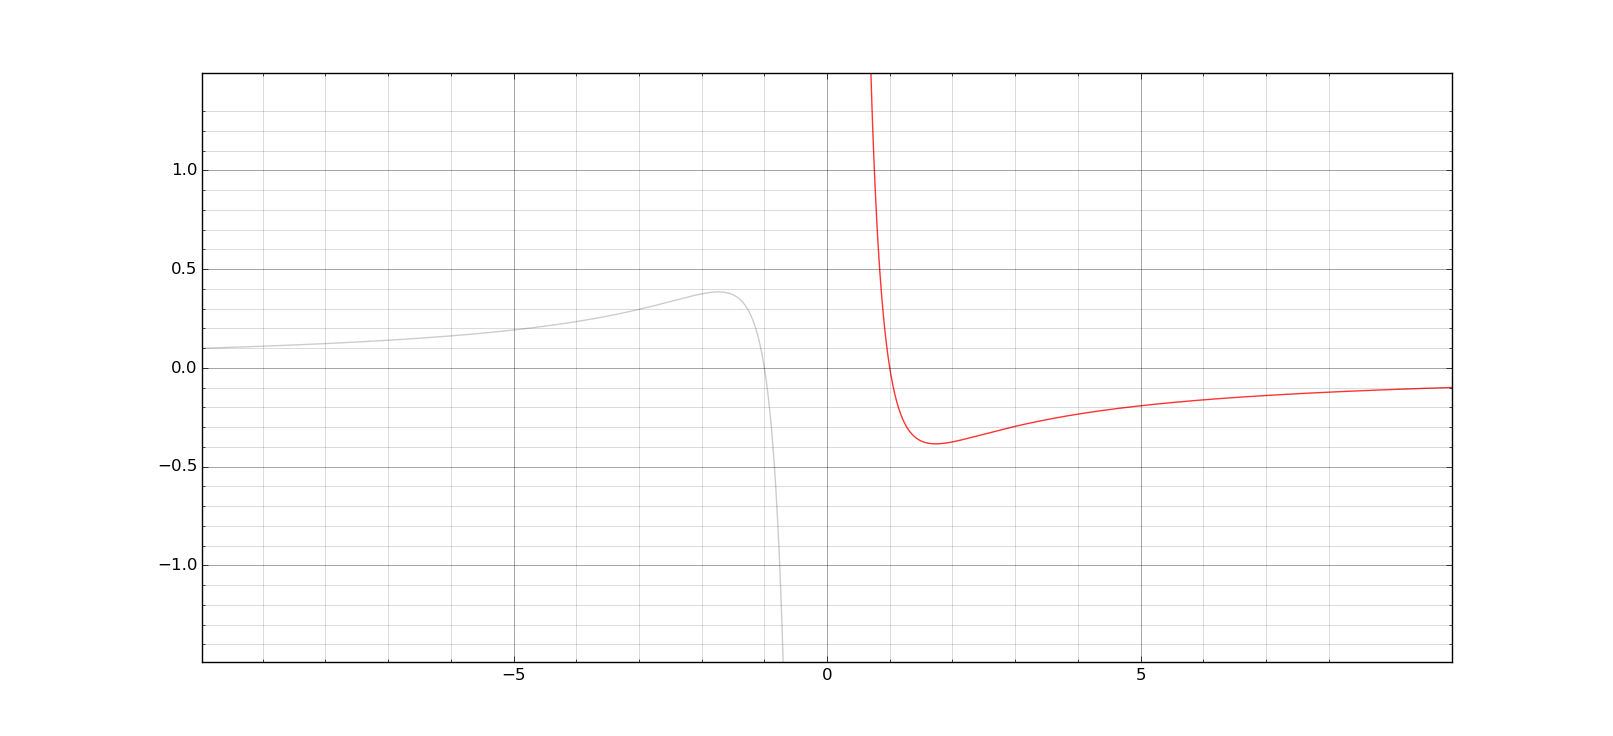
\includegraphics[width=0.8\textwidth, angle=0]{sigma_fn.png}
	   \caption{\(f(x)=\frac{1}{x^3}-\frac{1}{x}\), similar to \(\frac{\partial}{\partial \sigma}\mathcal{L}\)}
	   \label{fig1}
         \end{figure}

         \subsection*{iv)}
         Summarizing, \textbf{the maximum-likelihood estimators are}:
         \begin{equation*}
           \begin{split}
             &\hat\mu = \frac{1}{N}\sum_{n=1}^{N}\{x_n\} = \overline{X}\\
             &\hat\sigma^2 = \frac{1}{N}\sum_{n=1}^{N}\{(x_n-\hat\mu)^2\}
             \end{split}
         \end{equation*}







        \vspace{5mm}
	\section*{Exercise 3}
                 {\it please see/execute the python2 script ``fernandez\_blatt2.py'' for the specifities. }

                 \begin{figure}[ht]
	   \centering
           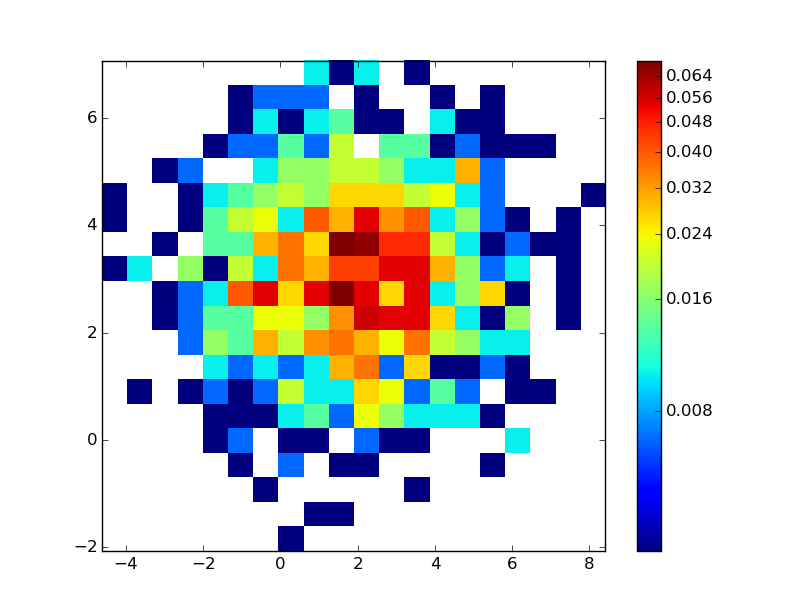
\includegraphics[width=0.8\textwidth, angle=0]{histogram_2D.png}
	   \caption{2D-histogram for 20x20 bins, 1000 samples}
	   \label{fig2}
                 \end{figure}
                 \begin{figure}[ht]
	   \centering
           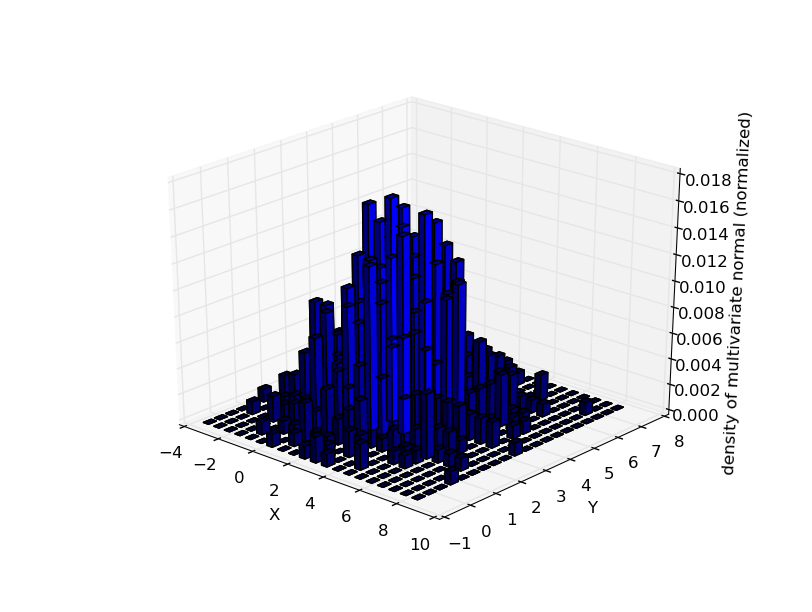
\includegraphics[width=0.8\textwidth, angle=0]{histogram_3D.png}
	   \caption{3D-histogram for 20x20 bins, 1000 samples}
	   \label{fig3}
         \end{figure}
                 
                 \subsection*{i) {\it real parameters: mean_x = 2, mean_y = 4, variance_x =4, variance_y = 2}}
                 To see how close the estimators are to the real parameters, simply substract them to their corresponding one. It is easy to see that the more samples were produced, the more precise the estimation is.\\[5mm]
        estimated mean of x for 1000 samples: 2.15392196764\\
        estimated mean of y for 1000 samples: 2.97162621077\\
        estimated variance of x for 1000 samples: 4.10347564674\\
        estimated variance of y for1000 samples: 2.00903592006\\
        estimated cov(x, y) for 1000 samples: -0.021877354475\\[5mm]
        estimated mean of x for 2 samples: 3.48570375761\\
        estimated mean of y for 2 samples: 0.855078387521\\
        estimated variance of x for 2 samples: 0.673930874005\\
        estimated variance of y for2 samples: 1.90147554895e-07\\
        estimated cov(x, y) for 2 samples: -0.987359761245\\[5mm]
        estimated mean of x for 20 samples: 2.00929953147\\
        estimated mean of y for 20 samples: 2.48505591435\\
        estimated variance of x for 20 samples: 2.06598830411\\
        estimated variance of y for20 samples: 1.66293241005\\
        estimated cov(x, y) for 20 samples: -1.6741426778\\[5mm]
        estimated mean of x for 200 samples: 2.10126575922\\
        estimat ed mean of y for 200 samples: 3.06414090786\\
        estimated variance of x for 200 samples: 4.03243403209\\
        estimated variance of y for200 samples: 1.78342385242\\
        estimated cov(x, y) for 200 samples: -0.310996676007\\[5mm]
        We see also that the estimated covariance tends to zero, the more samples we use.

	\vspace{5mm}
        \section*{Exercise 4}
        {\it Show that an arbitrary square matrix with elements \(w_{ij}\) can be written in the form \(w_{ij}\) = \(w_{ij}^S+w_{ij}^A\) where \(w_{ij}^S\) and \(w_{ij}^A\) are symmetric and anti-symmetric matrices, respectively, satisfying \(w_{ij}^S=w_{ji}^S\) and \(w_{ij}^A=-w_{ji}^A\) for all \(i\) and \(j\).}
        \subsection*{}
        %% The problem can be reformuled as follows: given three matrices:
        %% \begin{equation}\label{eq:20}
        %%     A,B,W \in \mathbb{R^{N\times N}} : a_{ij} = a_{ji} \;\;\text{and}\;\;b_{ij} = b_{ji} \;\;\;\;\forall i,j\in \{1,2,...,N\}
        %% \end{equation}
        %% Show that \(\)
        \(W \in \mathbb{R}^{N\times N}\) is an arbitrary square matrix when none of its elements has to satisfy any other property than being in \(\mathbb{R}\). Therefore, it suffices to show that 
        \begin{equation}\label{eq:20}
            (w_{ij}^S+w_{ij}^A = w_{ij}) \;\;\text{and}\;\; (w_{ij}^S-w_{ij}^A = w_{ji}) \quad : \quad w_{ij}^S,w_{ij}^A,w_{ij},w_{ji} \in \mathbb{R}
        \end{equation}
        Which can be easily done after the following transformations:
        \begin{equation*}
          \begin{split}
            &w_{ij}^S+w_{ij}^A = w_{ij} \iff w_{ij}^S = w_{ij}-w_{ij}^A\\
            &w_{ij}^S-w_{ij}^A = w_{ji} \iff w_{ij}^S = w_{ji}+w_{ij}^A\\
            &\iff w_{ij}-w_{ij}^A = w_{ji}+w_{ij}^A \iff 2w_{ij}^A = w_{ij}-w_{ji} \iff w_{ij}^A = \frac{w_{ij}-w_{ji}}{2}
          \end{split}
        \end{equation*}
        \begin{flushright}
          $\square$\\
        \end{flushright}


\vspace{5mm}
\section*{Exercise 5}
{\it Show that a real, symmetric matrix of size \(D\times D\) has \(D(D+1)/2\) independent parameters.}
\subsection*{i)}
The real matrix \(M\in \mathbb{R}^{D\times D}\) is symmetric when \(m_{ij}=m_{ji}\quad \forall i,j \in \{1,2,...,D\}\).\\
Further, independent parameters are those elements of \(M\) whose only constraint is that they have to be in \(\mathbb{R}\). This holds for every element on the matrix diagonal, since every real number holds the constraint \(m_{ii}=m_{ii}\). For every other element, it holds that
\begin{equation}
  m_{ij}\;\text{is independent} \iff m_{ji}\;\text{is NOT independent}\qquad \forall m_{ij},m_{ji} \in M
\end{equation}
Simply because both of them have to be equal. The criterium to select which one of them is the independent and which the dependent is undefined. For instance, if taking \((m_{ij}\;\text{is independent} \iff j<i)\) it can be nicely said that \textbf{every element in or above the diagonal is independent, and every other dependent}, which can be seen as the non-zero part of a triangular matrix. If counting its elements diagonally, we see that the biggest diagonal has \(D\) elements, and the diagonal size decreases by one:

\begin{equation}
\begin{pmatrix}
m_{11} & m_{12} & m_{13} & m_{14} \\
... & m_{22} & m_{23} & m_{24} \\
... & ... & m_{33} & m_{34} \\
... & ... & ... & m_{44}
\end{pmatrix}
\end{equation}
Therefore, the total number of independent elements is given by the sum
\begin{equation}
  1+2+...+D = \sum_{d=1}^D\{d\}
\end{equation}
\subsection*{ii)}
It remains to proof that \(\sum_{d=1}^D\{d\} = \frac{D(D+1)}{2}\), which can be done in different ways. One very intuitive way, attributed to Gauss when he was still at primary school, is to (ab)use addition's commutative property:
\begin{equation}
  \sum_{d=1}^D\{d\} = 1+2+...+D = \underbrace{(1+D),(2+(D-1)), ..., (\overline{D})}_{\frac{D}{2} \text{ times}} = (D+1)\frac{D}{2} =  \frac{D(D+1)}{2}  
\end{equation}
Whereas \(\overline{D} =\(\frac{D}{2}+(\frac{D}{2}+1) = D+1\)
\begin{flushright}
  $\square$\\
\end{flushright}






\end{document}
